\documentclass{article}
\usepackage{fancyhdr}
\usepackage{xeCJK}
\usepackage{pifont}
\usepackage{graphicx}
\usepackage{float}
\usepackage{geometry}
\geometry{left=1.5cm,right=1.5cm,top=3cm,bottom=3cm}
%\setmainfont{Times New Roman}  
\setCJKmainfont{Songti SC}
\pagestyle{fancy}
\fancypagestyle{plain}{
    \fancyhf{}
    \fancyfoot[C]{\thepage}
    \renewcommand\headrulewidth{0pt}
}
\begin{document}
    \noindent\textbf{3.5}\par
    \ding{172}主存储器简称内存,是计算机运行时的存储主力。一般存储运行时的指令、各种运行变量、外部文件的指针等。计算机中的程序运行都是在主存中进行的。\par
    \ding{173}外存储器不易丢失,主要用来存储需要永久存储的文件。联机外存一般为磁介质的机械硬盘或者固态硬盘;脱机外存便于携带,如u盘等。
    \\[4pt]\par

    \noindent\textbf{3.6}\par
    \ding{172}IDE接口\par
    \ding{173}SCSI接口\par
    \ding{174}SATA和SAS接口\par
    \ding{175}SD接口\par
    \ding{176}eMMC接口
    \\[4pt]\par

    \noindent\textbf{3.8}\par
    三种存储器中的信息不易失,可以长久保存;都可以多次编程写入数据\par
    原因:三种存储器种的信息都能稳定存储,可以长久保存,需要用紫外线或者电信号进行擦除,适合用作只读存储器。
    \\[4pt]\par

    \noindent\textbf{3.10}\par
    \ding{172}内存带宽不断加大:前三代带宽翻倍,到DDR4提升了bank数量\par
    \ding{173}工作电压下降,功耗降低\par
    \ding{174}集成度变高,单根内存条容量增加\par
    \ding{175}插槽设计优化,提高工作稳定性和拆除的便利性\par
    \ding{176}支持的工作主频率变高,工作效率提升
    \\[4pt]\par

    \noindent\textbf{3.12}\par
    \ding{172}确保可以运行需求空间比实际主存更大的程序\par
    \ding{173}确保可执行程序装载后内存空间的连续\par
    \ding{174}确保同时加载多个程序的时候内存地址不会冲突
    \\[4pt]\par

    \noindent\textbf{3.16}\par
    原理:在主存和CPU之间放置一块高速的SRAM存储器,将近期重复执行的内存信息存入其中,访问时如果在里面就直接取出,不需要经过主存读取。\par
    作用:提高CPU访问主存储器的速度和效率。\par
    适用场景:CPU大量重复地访问小范围局部信息时、Cache的命中率会较高
    \\[4pt]\par

    \noindent\textbf{3.17}\par
    原因:Cache本身是局部内存的一份副本,内容需要保持和内存值一致,否则读取时会出现逻辑的错误。\par
    方法:\par
    \qquad\ding{172}写通方式:写信号发送到Cache时,也直接写入主存\par
    \qquad\ding{173}写回方式:收到写信号时只改变Cache中的值,并设标志位为1;当此块Cache要移出且标志位为1时才修改主存
    \\[4pt]\par

    \noindent\textbf{3.22}\par
    见最后一页\par
    使用3-8译码器来对地址进行译码\par
    译码器连接每个存储器对使能端,表示这个存储器可用
    \\
    \begin{figure}[h]
        \centering
        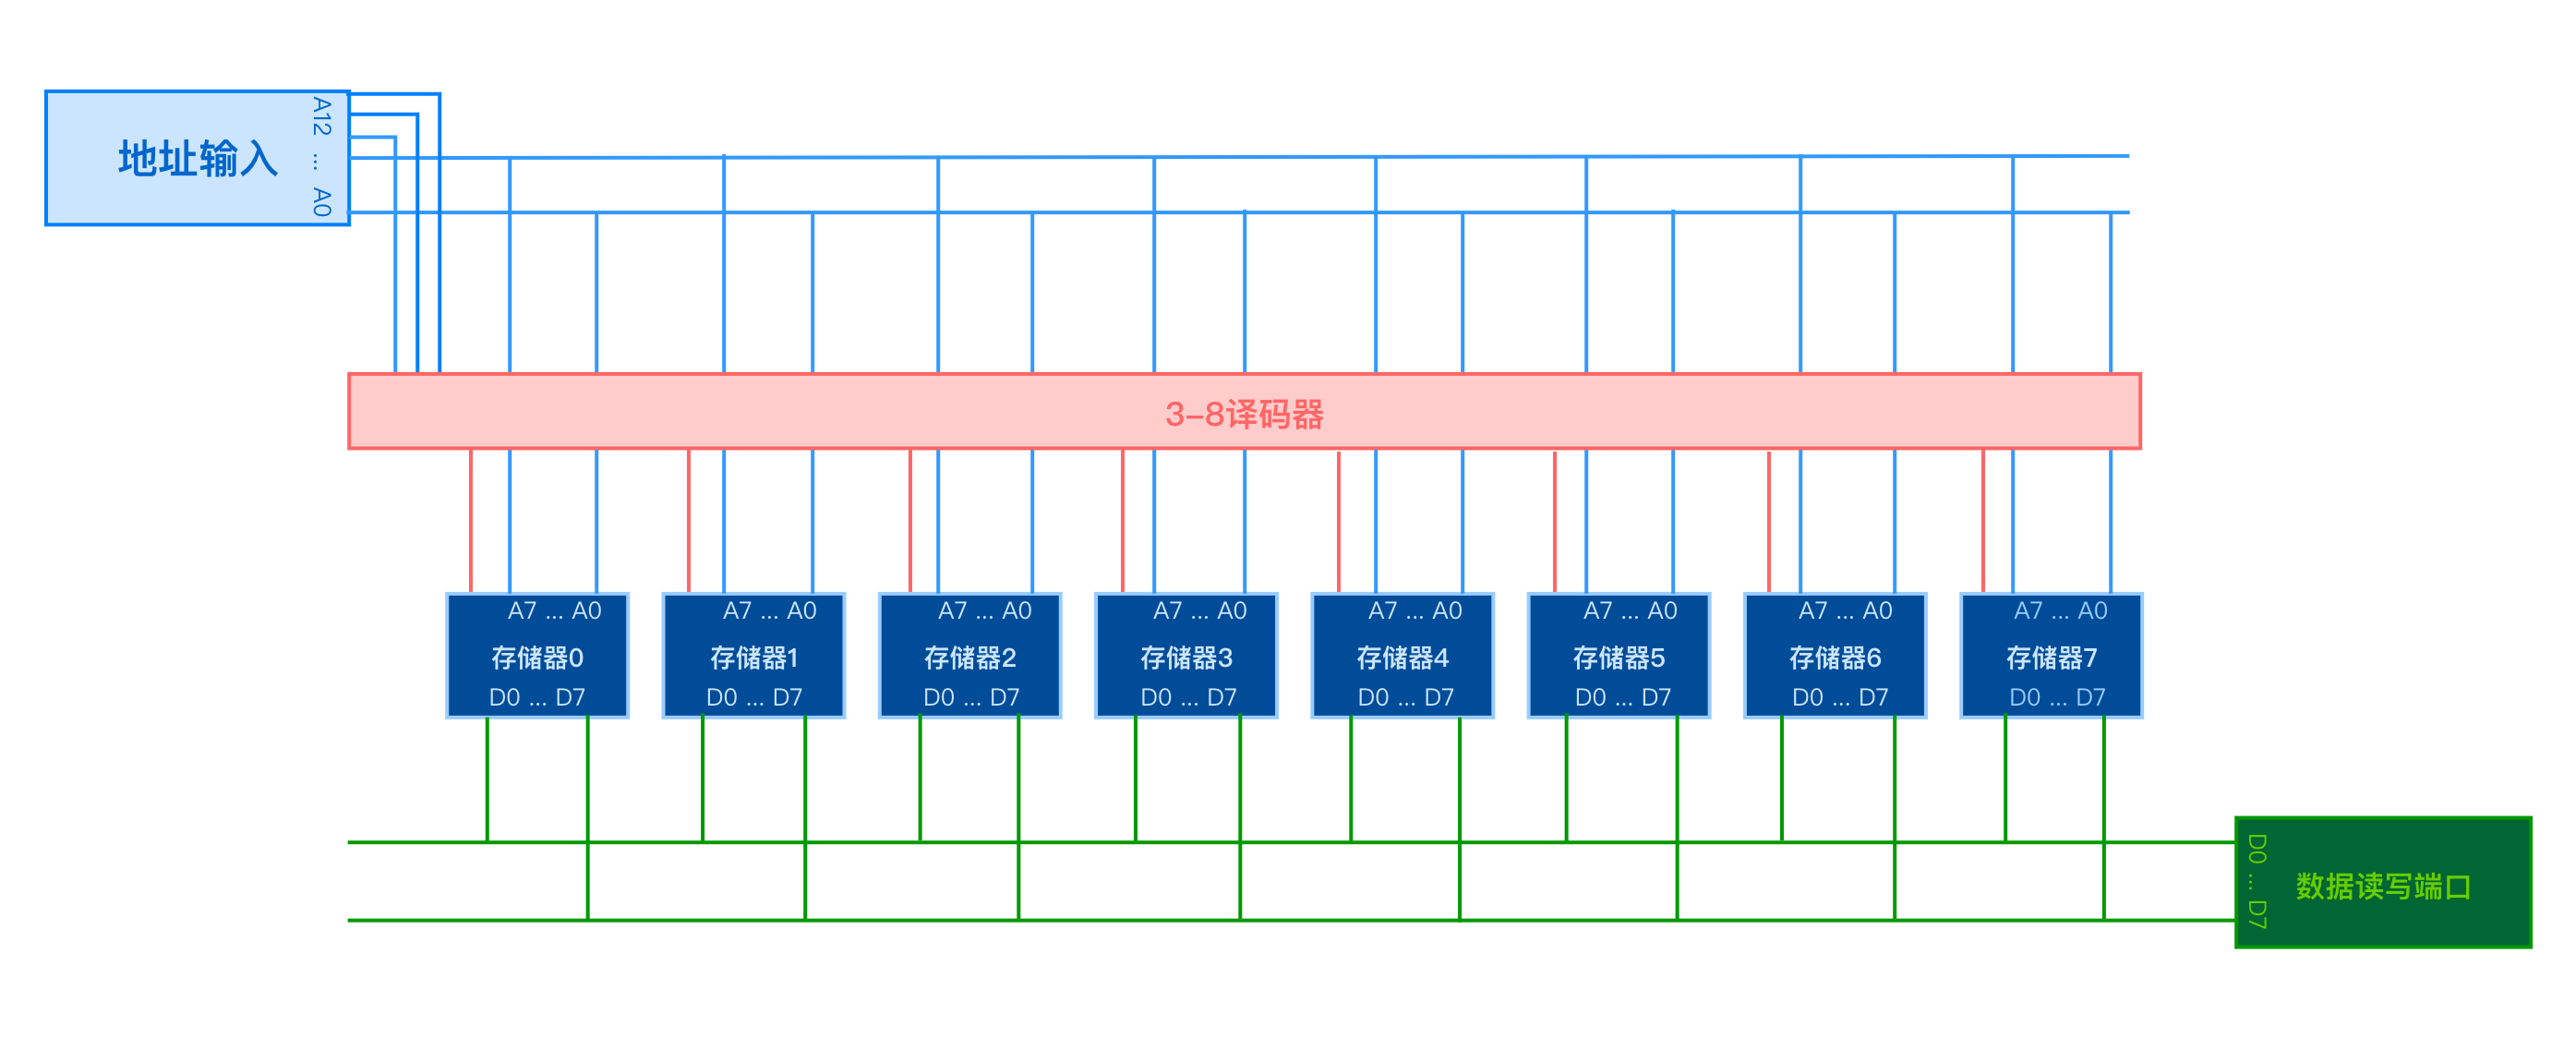
\includegraphics[scale=0.18]{hw3.png}
    \end{figure}
    \\[4pt]\par

    \noindent\textbf{3.22}\par
    需要根据实际的主存容量、芯片粒数、单元数、芯片位宽与Bank之间的关系进行扩展。
    \\[4pt]\par

\end{document}